\graphicspath{{images_low_res/}}
\section{Approach}
\label{sec:approach}

\subsection{Develop an Initial Model}
\label{sec:initial_model}



Figure~\ref{fig:simple_model} shows a schematic of our initial approach to modelling (nutrient dependent growth with nutrient and signal diffusion).
Each culture on the agar is given a label, \(i\), and has three variables associated with it: \(C_{i}\), the observed culture size, and the hidden variables, \(N_{i}\), the amount of nutrients at location \(i\), and \(S_{i}\), the amount of signal molecule location \(i\).
Cultures in QFA and SGA agars are arranged in a square array, each culture having eight neighbours with which they could conceivably interact with directly. Initially, we will model diffusion between only the four closest neighbours, in the vertical and horizontal directions (darker blue circles in Figure~\ref{fig:simple_model}).
We will describe nutrient dependent growth at each location using mass action kinetics and the following reaction equation:
\begin{equation}
  \label{eq:1}
  C + N \xrightarrow[]{r_{i}} 2C
\end{equation}
As a first approach, assuming that the number of cells is continuous, we will incorporate the effect of signal molecules on growth and the diffusion of both nutrient and signal molecules using the following ODEs:
\begin{align}
  \label{eq:2}
  \frac{dC_{i}}{dt}& = r_{i}N_{i}C_{i} - \beta S_{i},\\
  \frac{dN_{i}}{dt}& = - r_{i}N_{i}C_{i} - k_{n}\sum_{j}(N_{i} - N_{j})\\
  \frac{dS_{i}}{dt}& = \alpha C_{i} - k_{s}\sum_{j}(S_{i} - S_{j})
\end{align}
where \(j\) indicates the closest neighbours.
If necessary, diagonal neighbours could be incorporated into this modelling approach using an additional or adjusted diffusion parameter. In section~\ref{sec:dev-mod-further} we discuss the possibility of using finer-grain spatially-discretised or continuous models of diffusion. Alternative models for signalling effect could be used; here we have chosen to use the simplest.
\begin{equation}
  \label{eq:3}
  \frac{dC_{i}}{dt}& = r_{i}N_{i}C_{i}(1 - \frac{S_{i}}{S_{crit}})
\end{equation}

Model reactions using mass action kinetics

Simulate ODE in p




\begin{Figure}
  \centering
  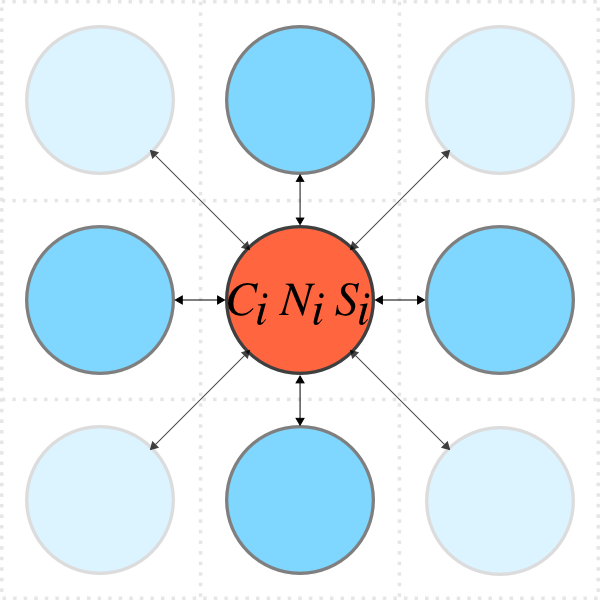
\includegraphics[width=\linewidth]{square_array}
  \captionof{figure}{Schematic of simple modelling approach.}
  \label{fig:simple_model}
\end{Figure}

\subsection{Analyse Experimental Data}
\label{sec:analyse-data}

\subsection{Develop Model Further}
\label{sec:dev-mod-further}

\begin{Figure}
  \centering
  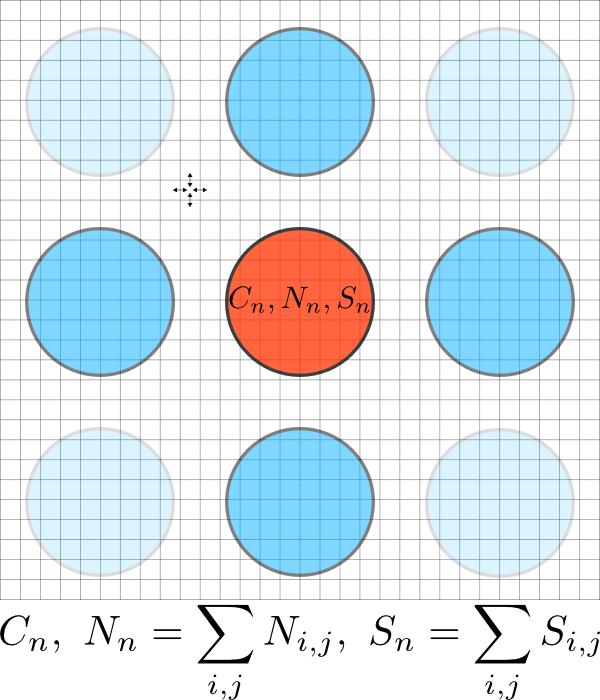
\includegraphics[width=\linewidth]{square_array_grid}
  \captionof{figure}{Schematic of a spatially-discretized two-dimensional model.}
\end{Figure}

\begin{Figure}
  \centering
  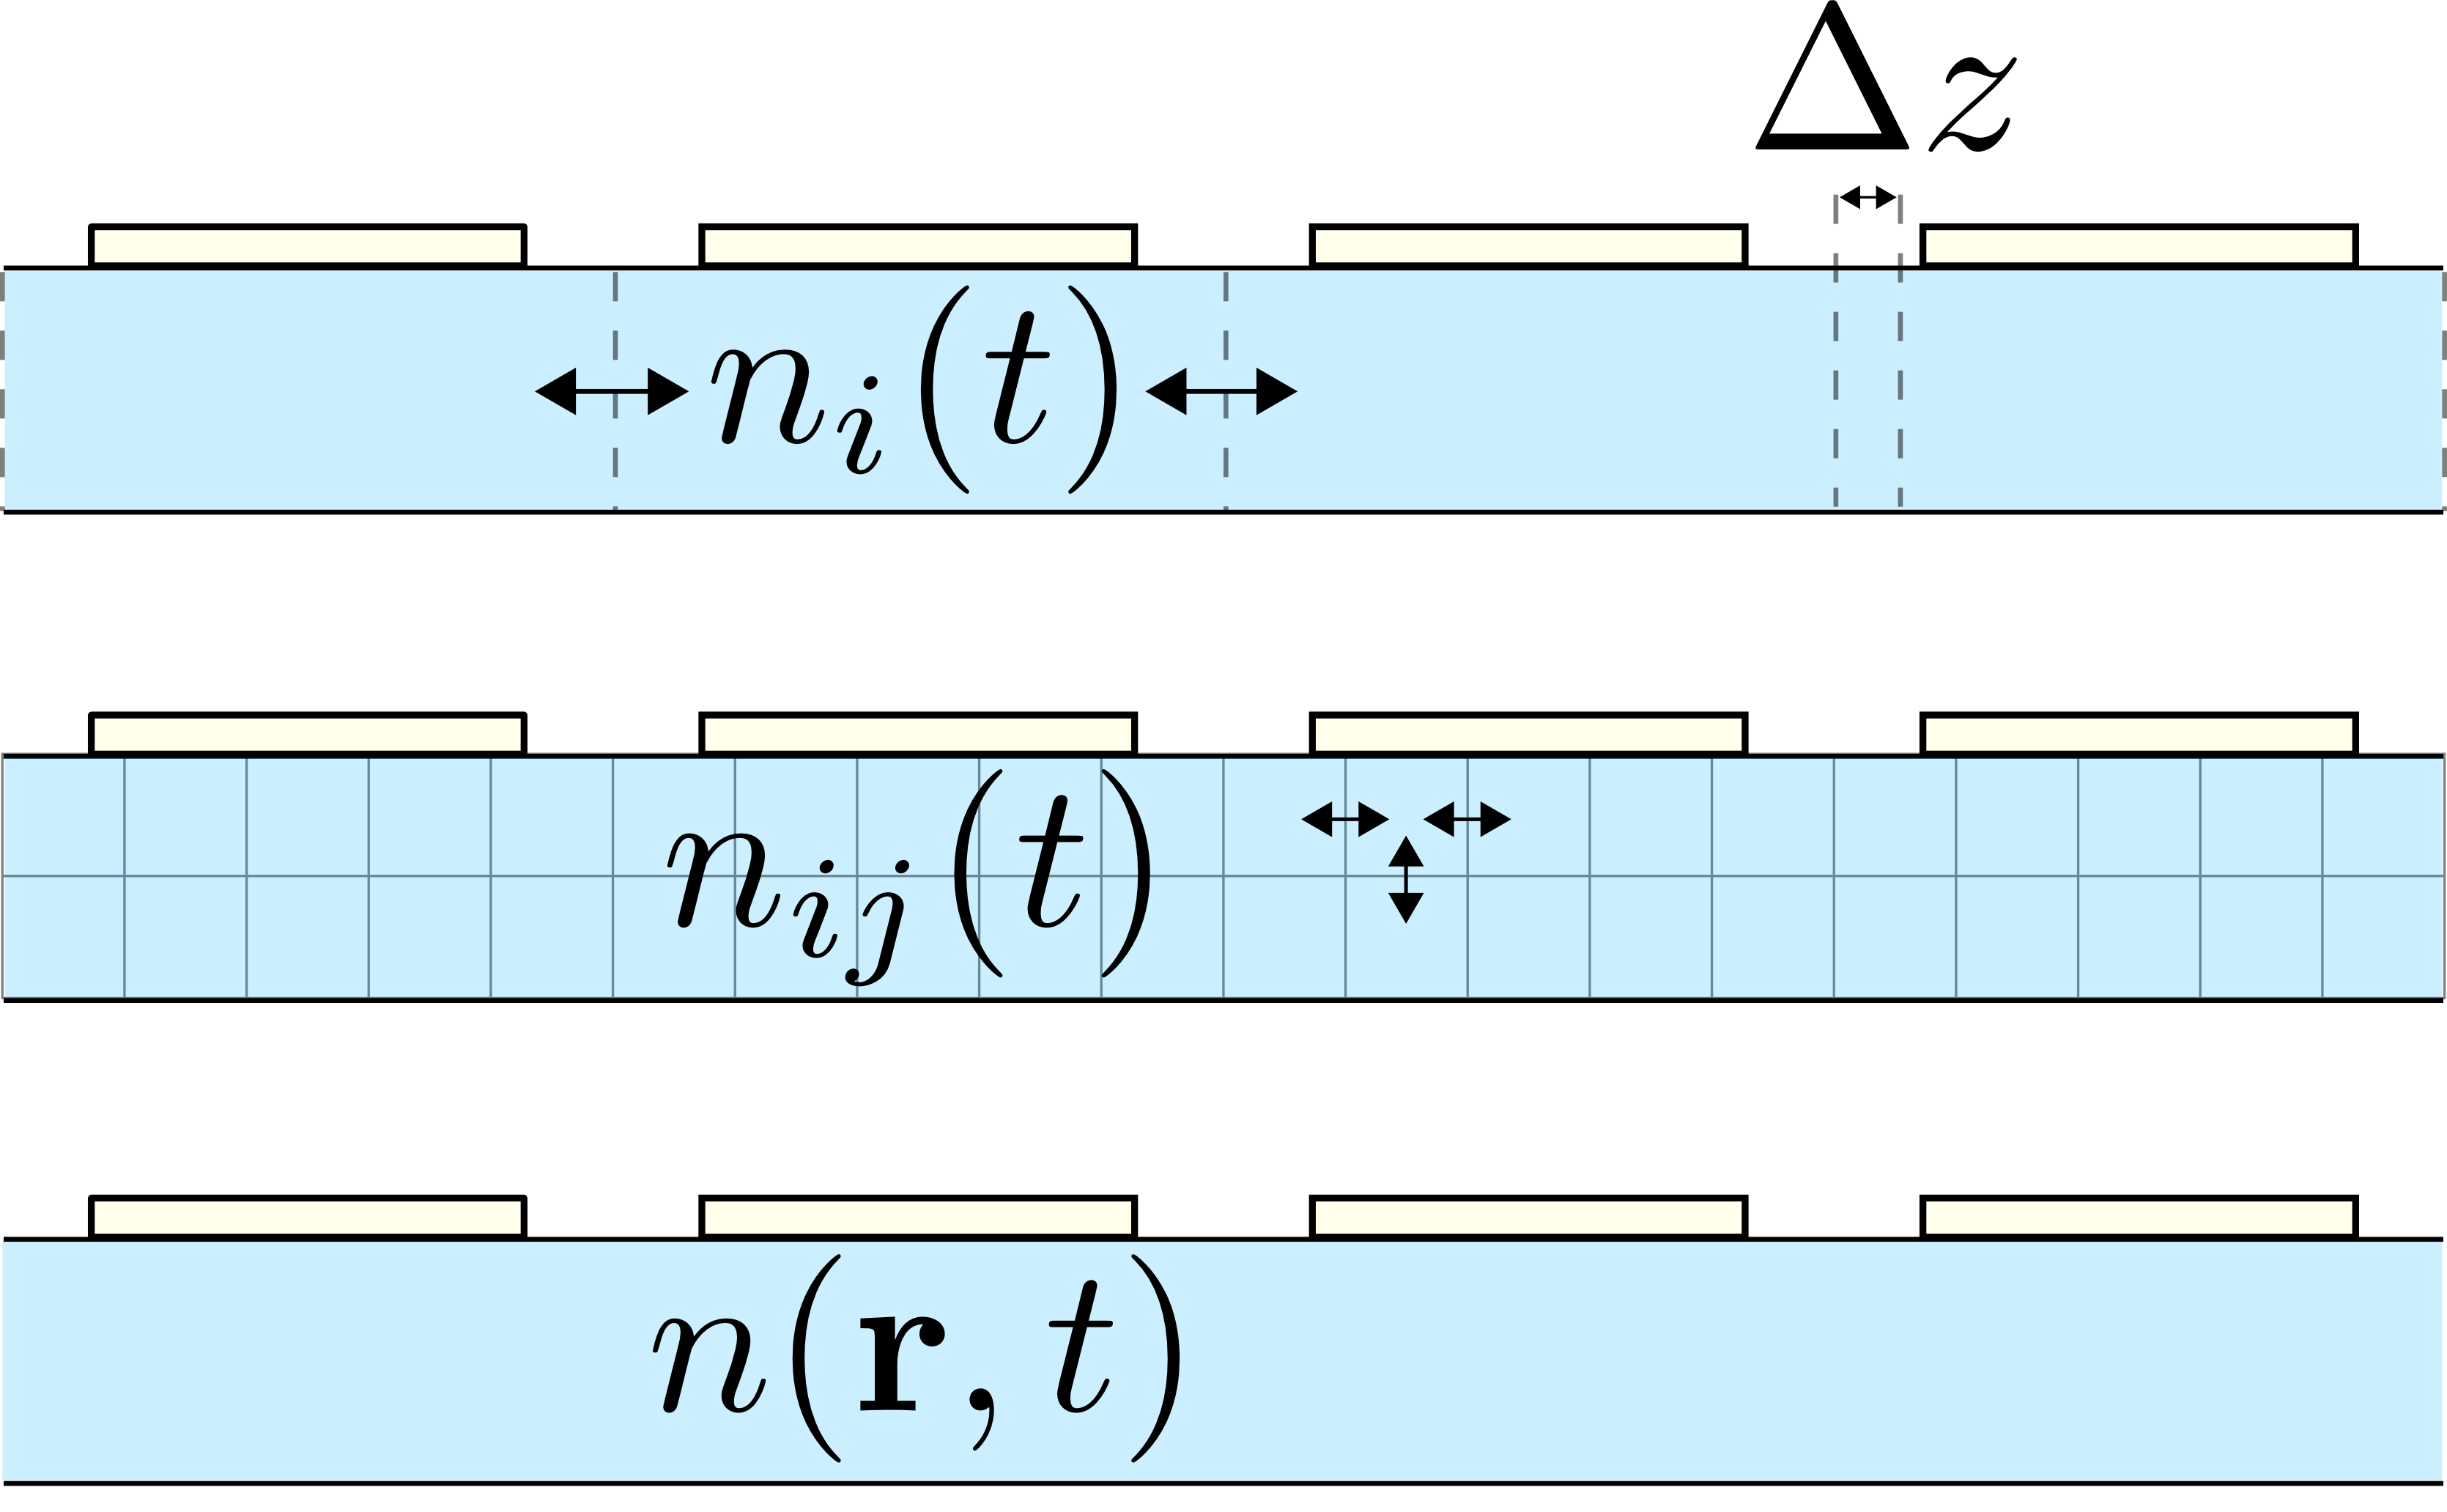
\includegraphics[width=\linewidth]{height_dep_miniqfa_delta_z}
  \captionof{figure}{Schematics of diffusion across agar height.}
\end{Figure}
% Could model movement of vertical or movement across it.
\subsection{Compare Experimental Designs}
\label{sec:comp-exper-designs}


\begin{Figure}
  \centering
  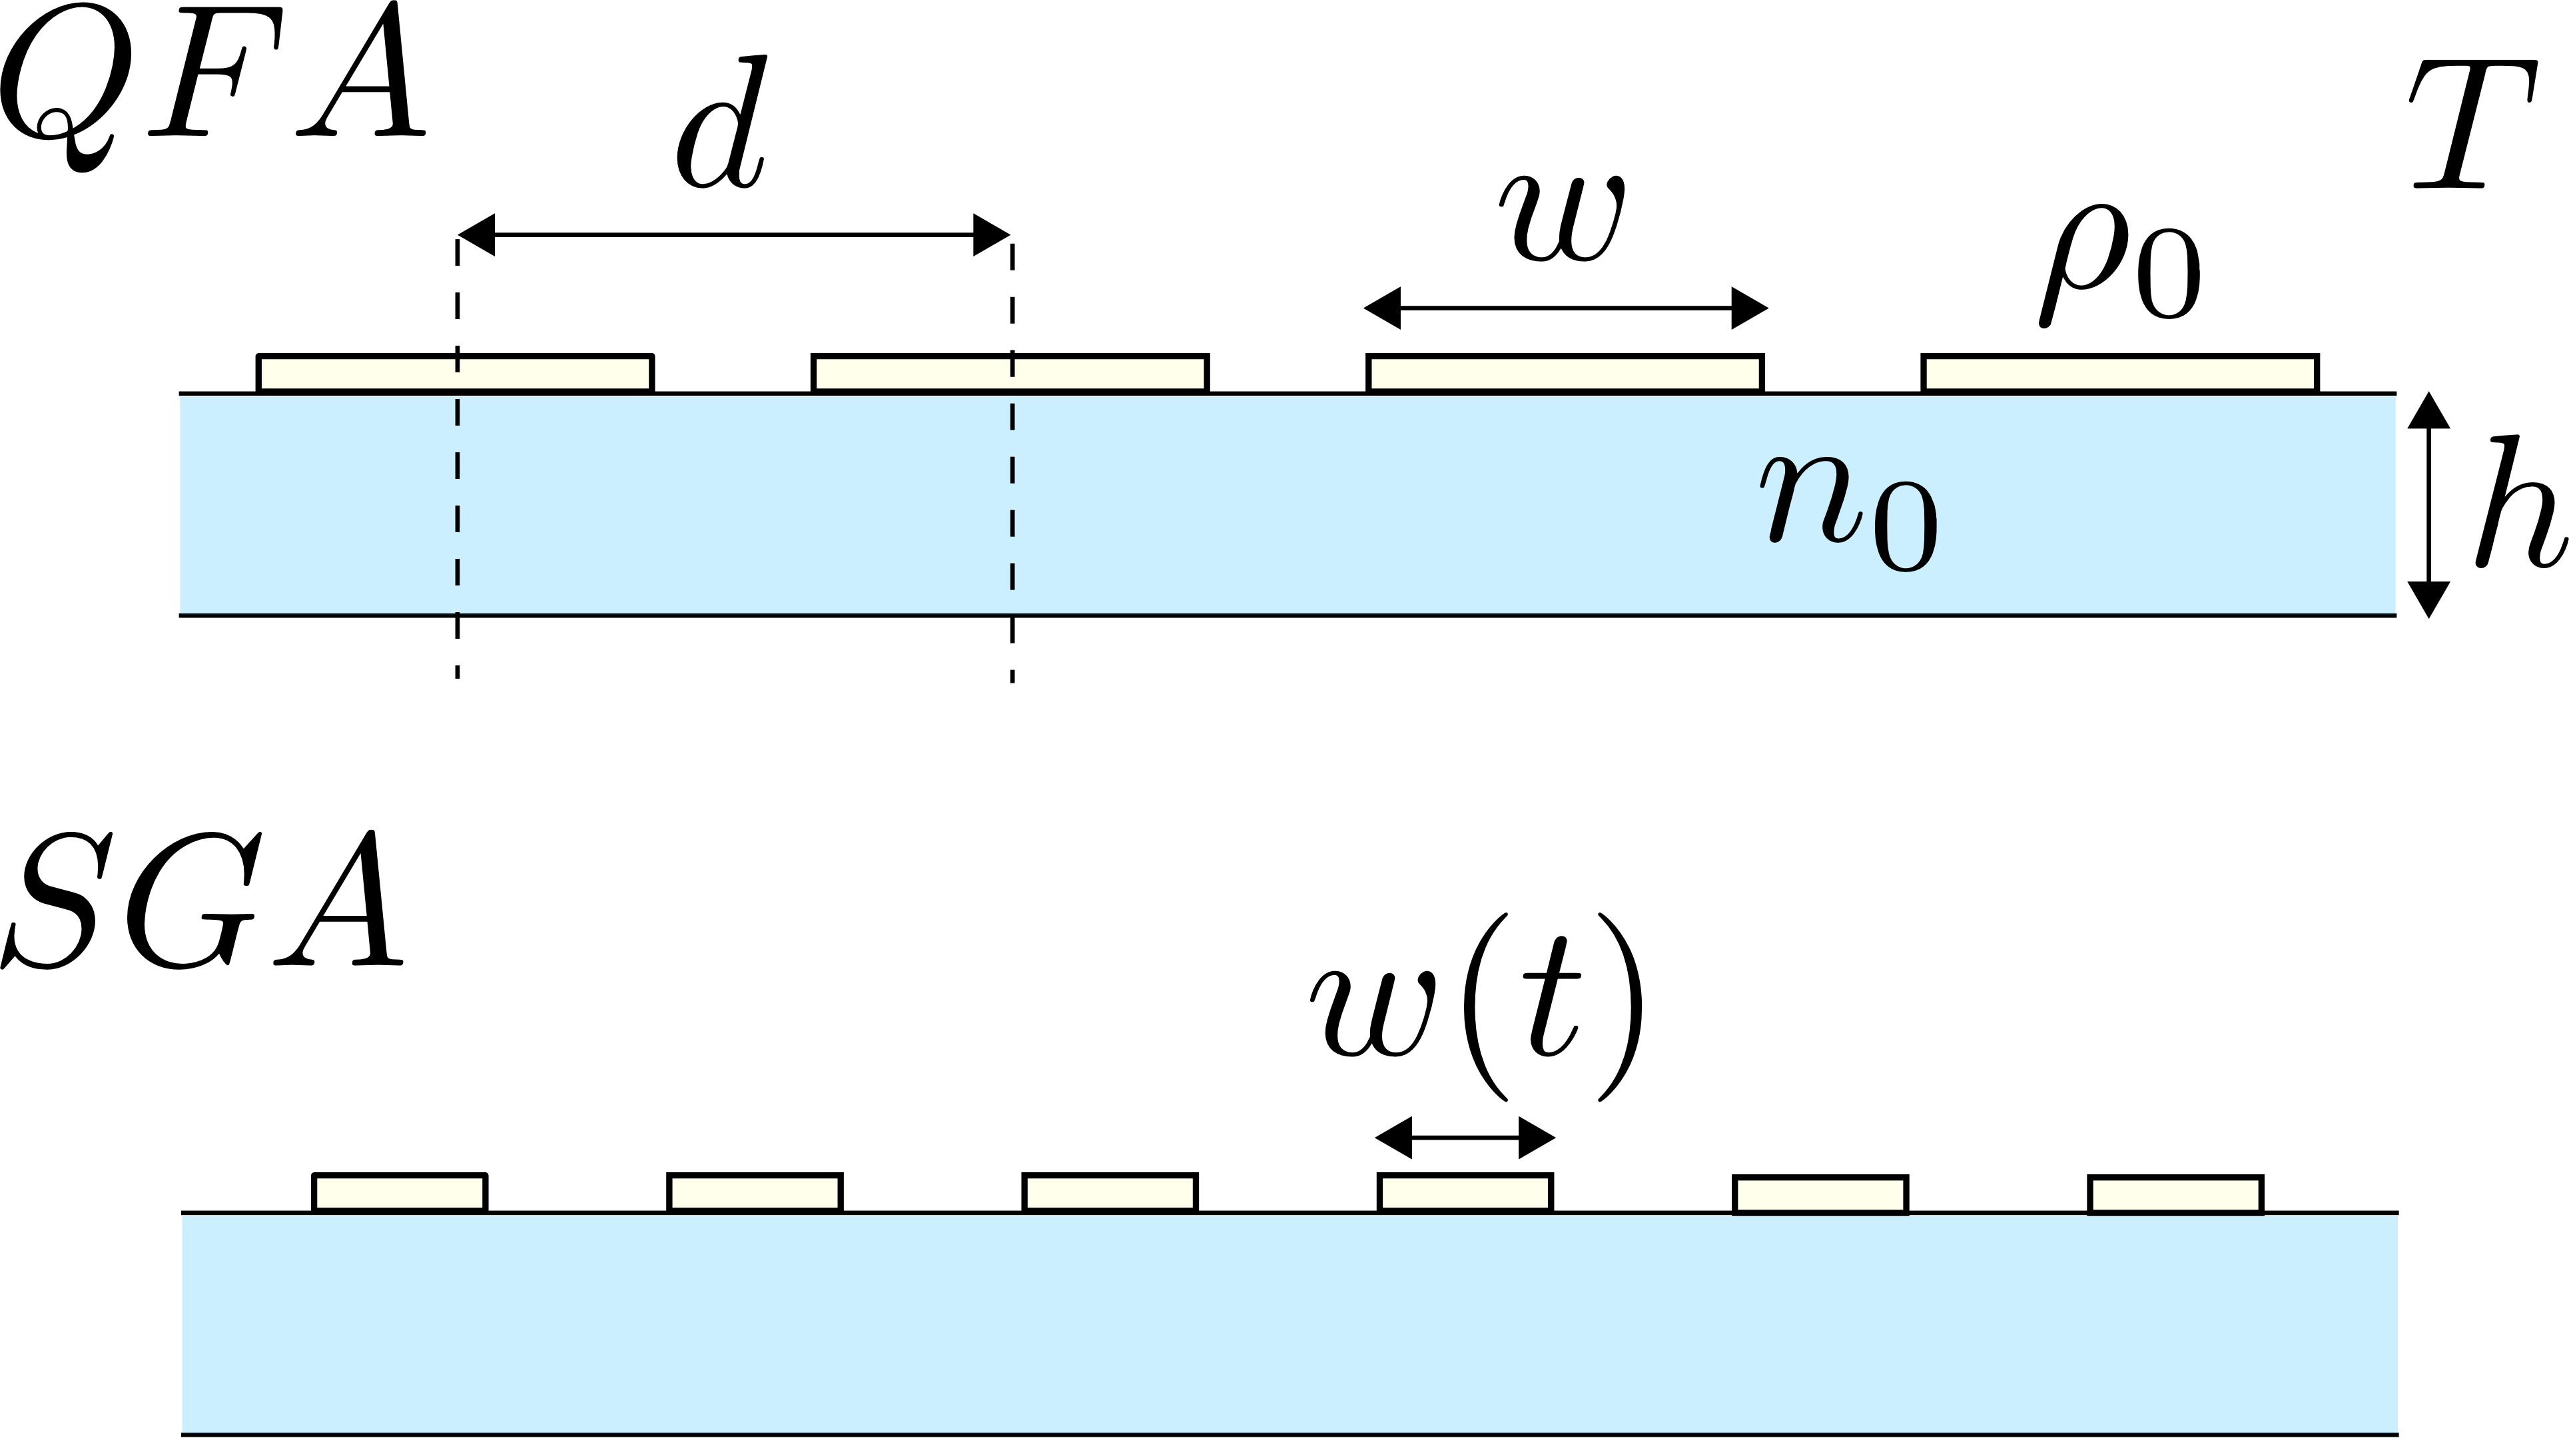
\includegraphics[width=\linewidth]{qfa_v_sga_vars}
  \captionof{figure}{QFA and SGA agars.}
\end{Figure}



\begin{Figure}
  \centering
  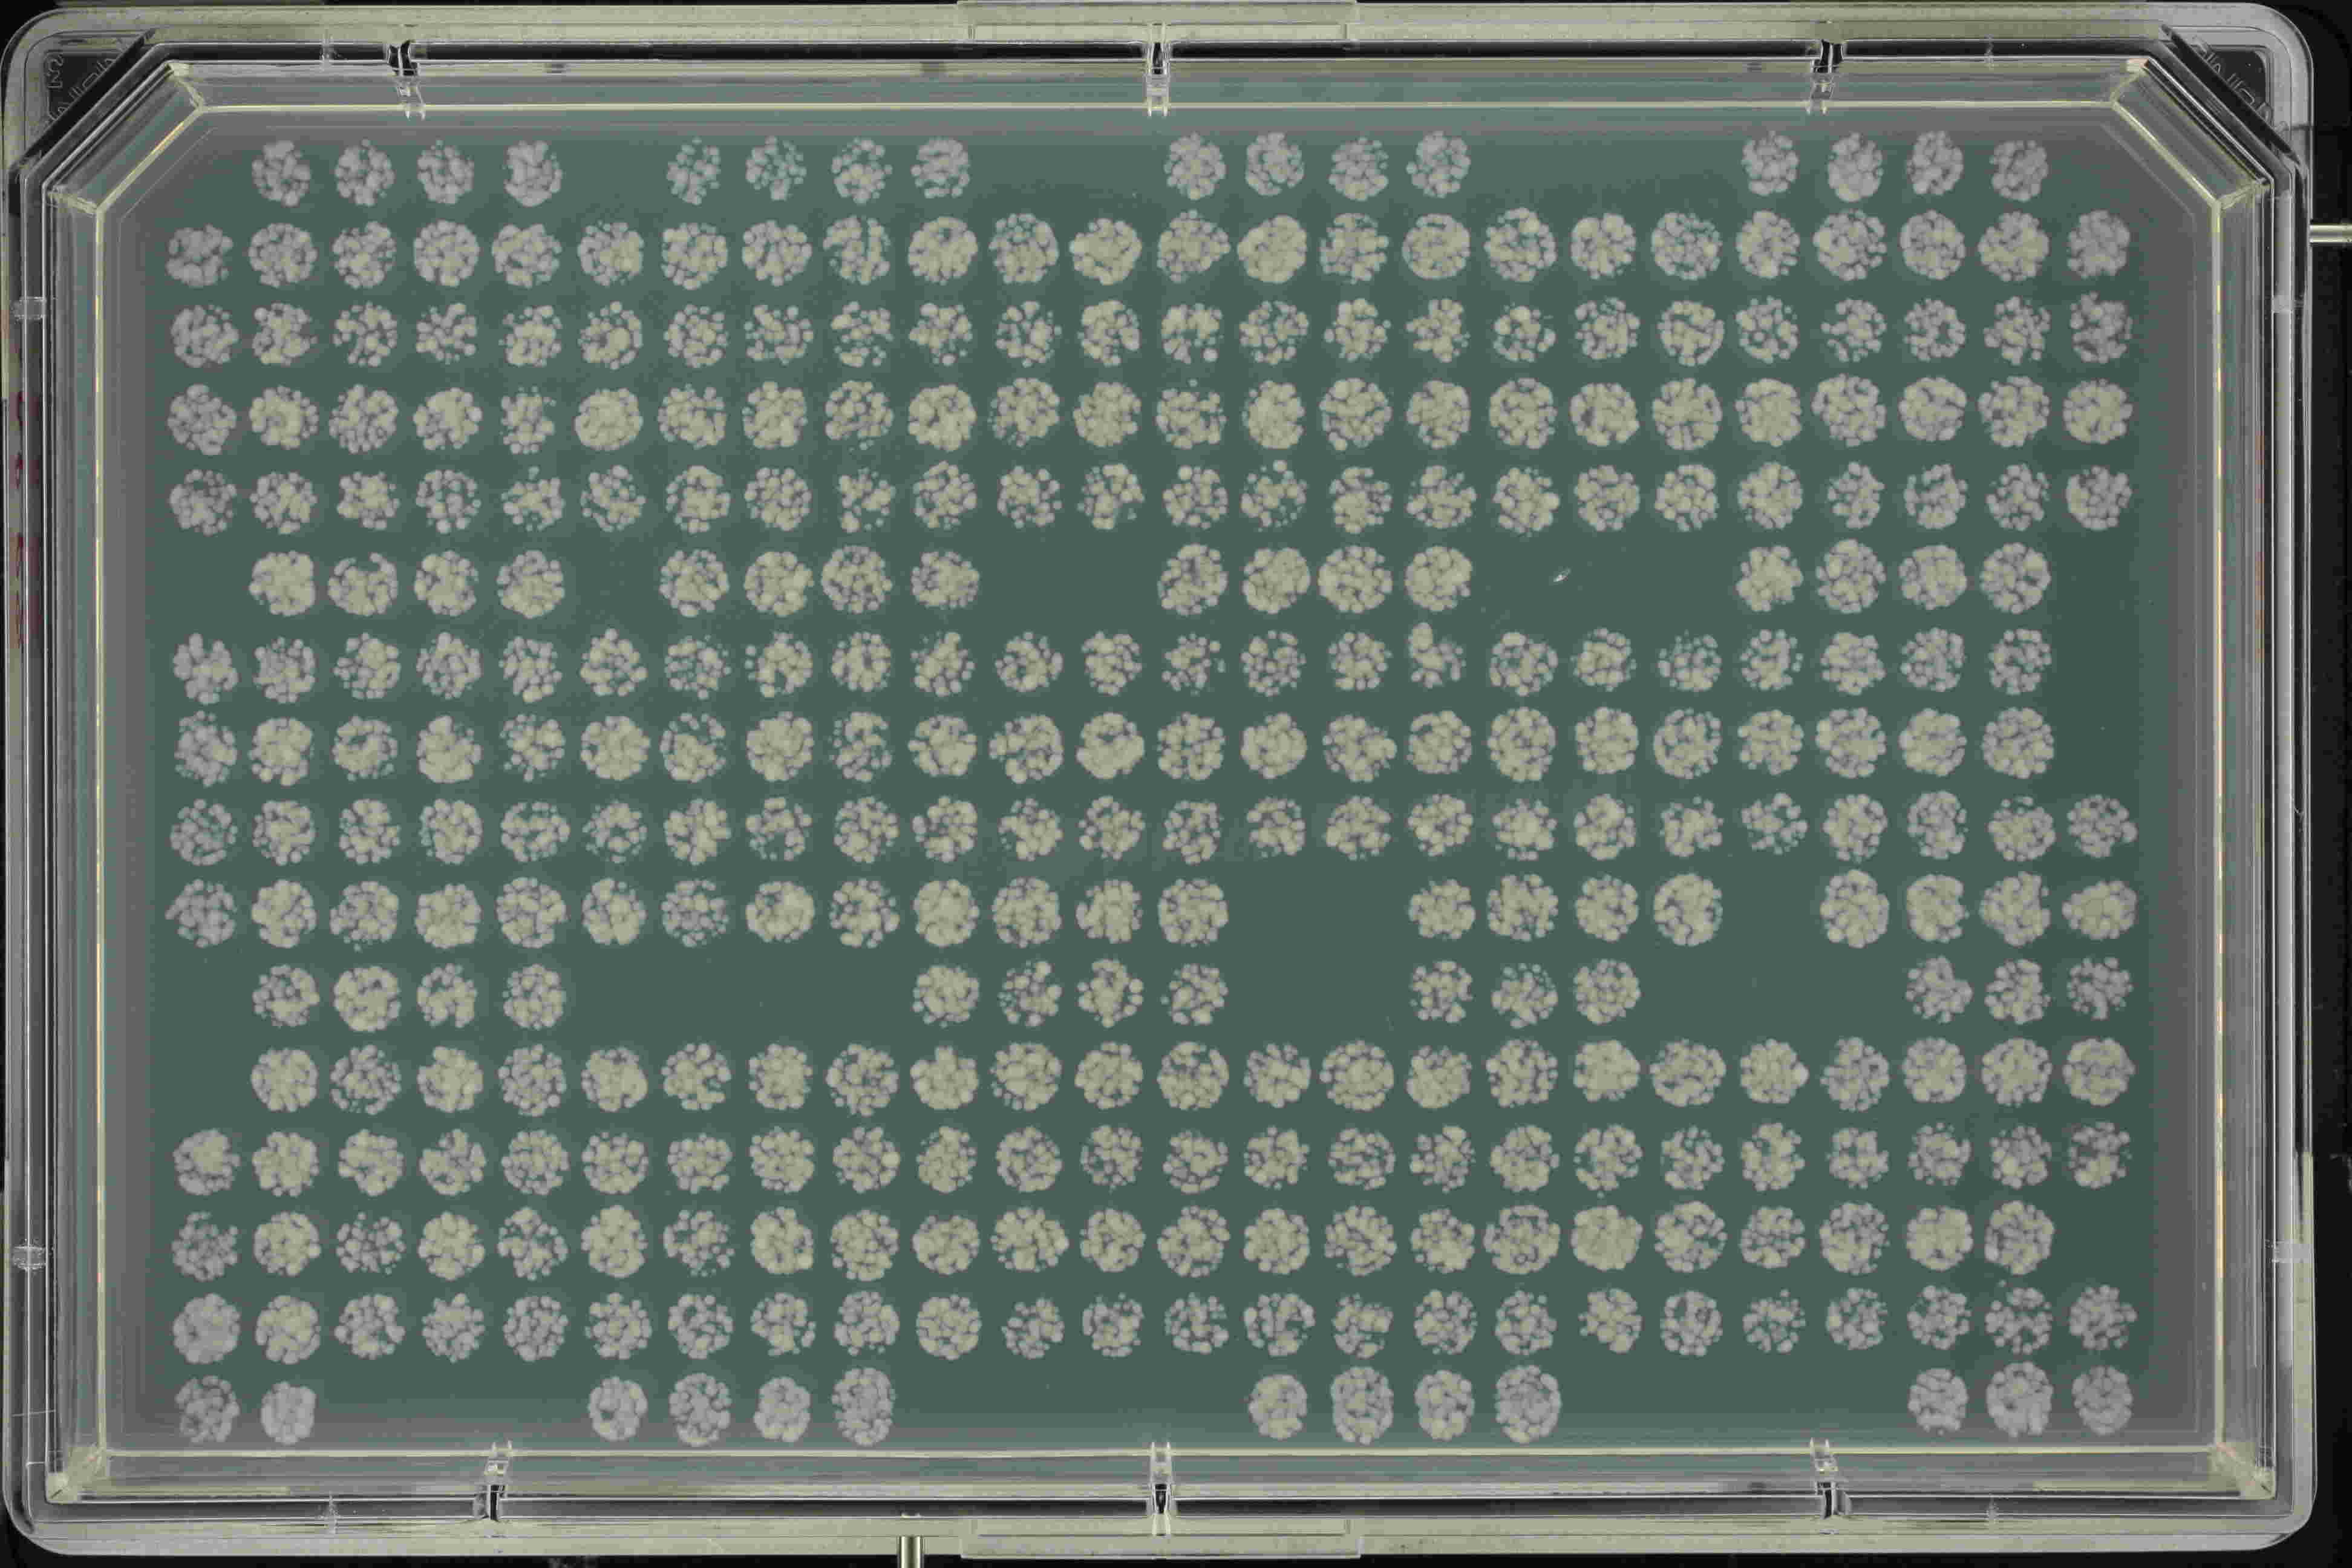
\includegraphics[width=\linewidth]{DLR00012647-2009-07-02_23-12-49}
  \captionof{figure}{Schematics of diffusion across agar height.}
\end{Figure}

\begin{Figure}
  \centering
  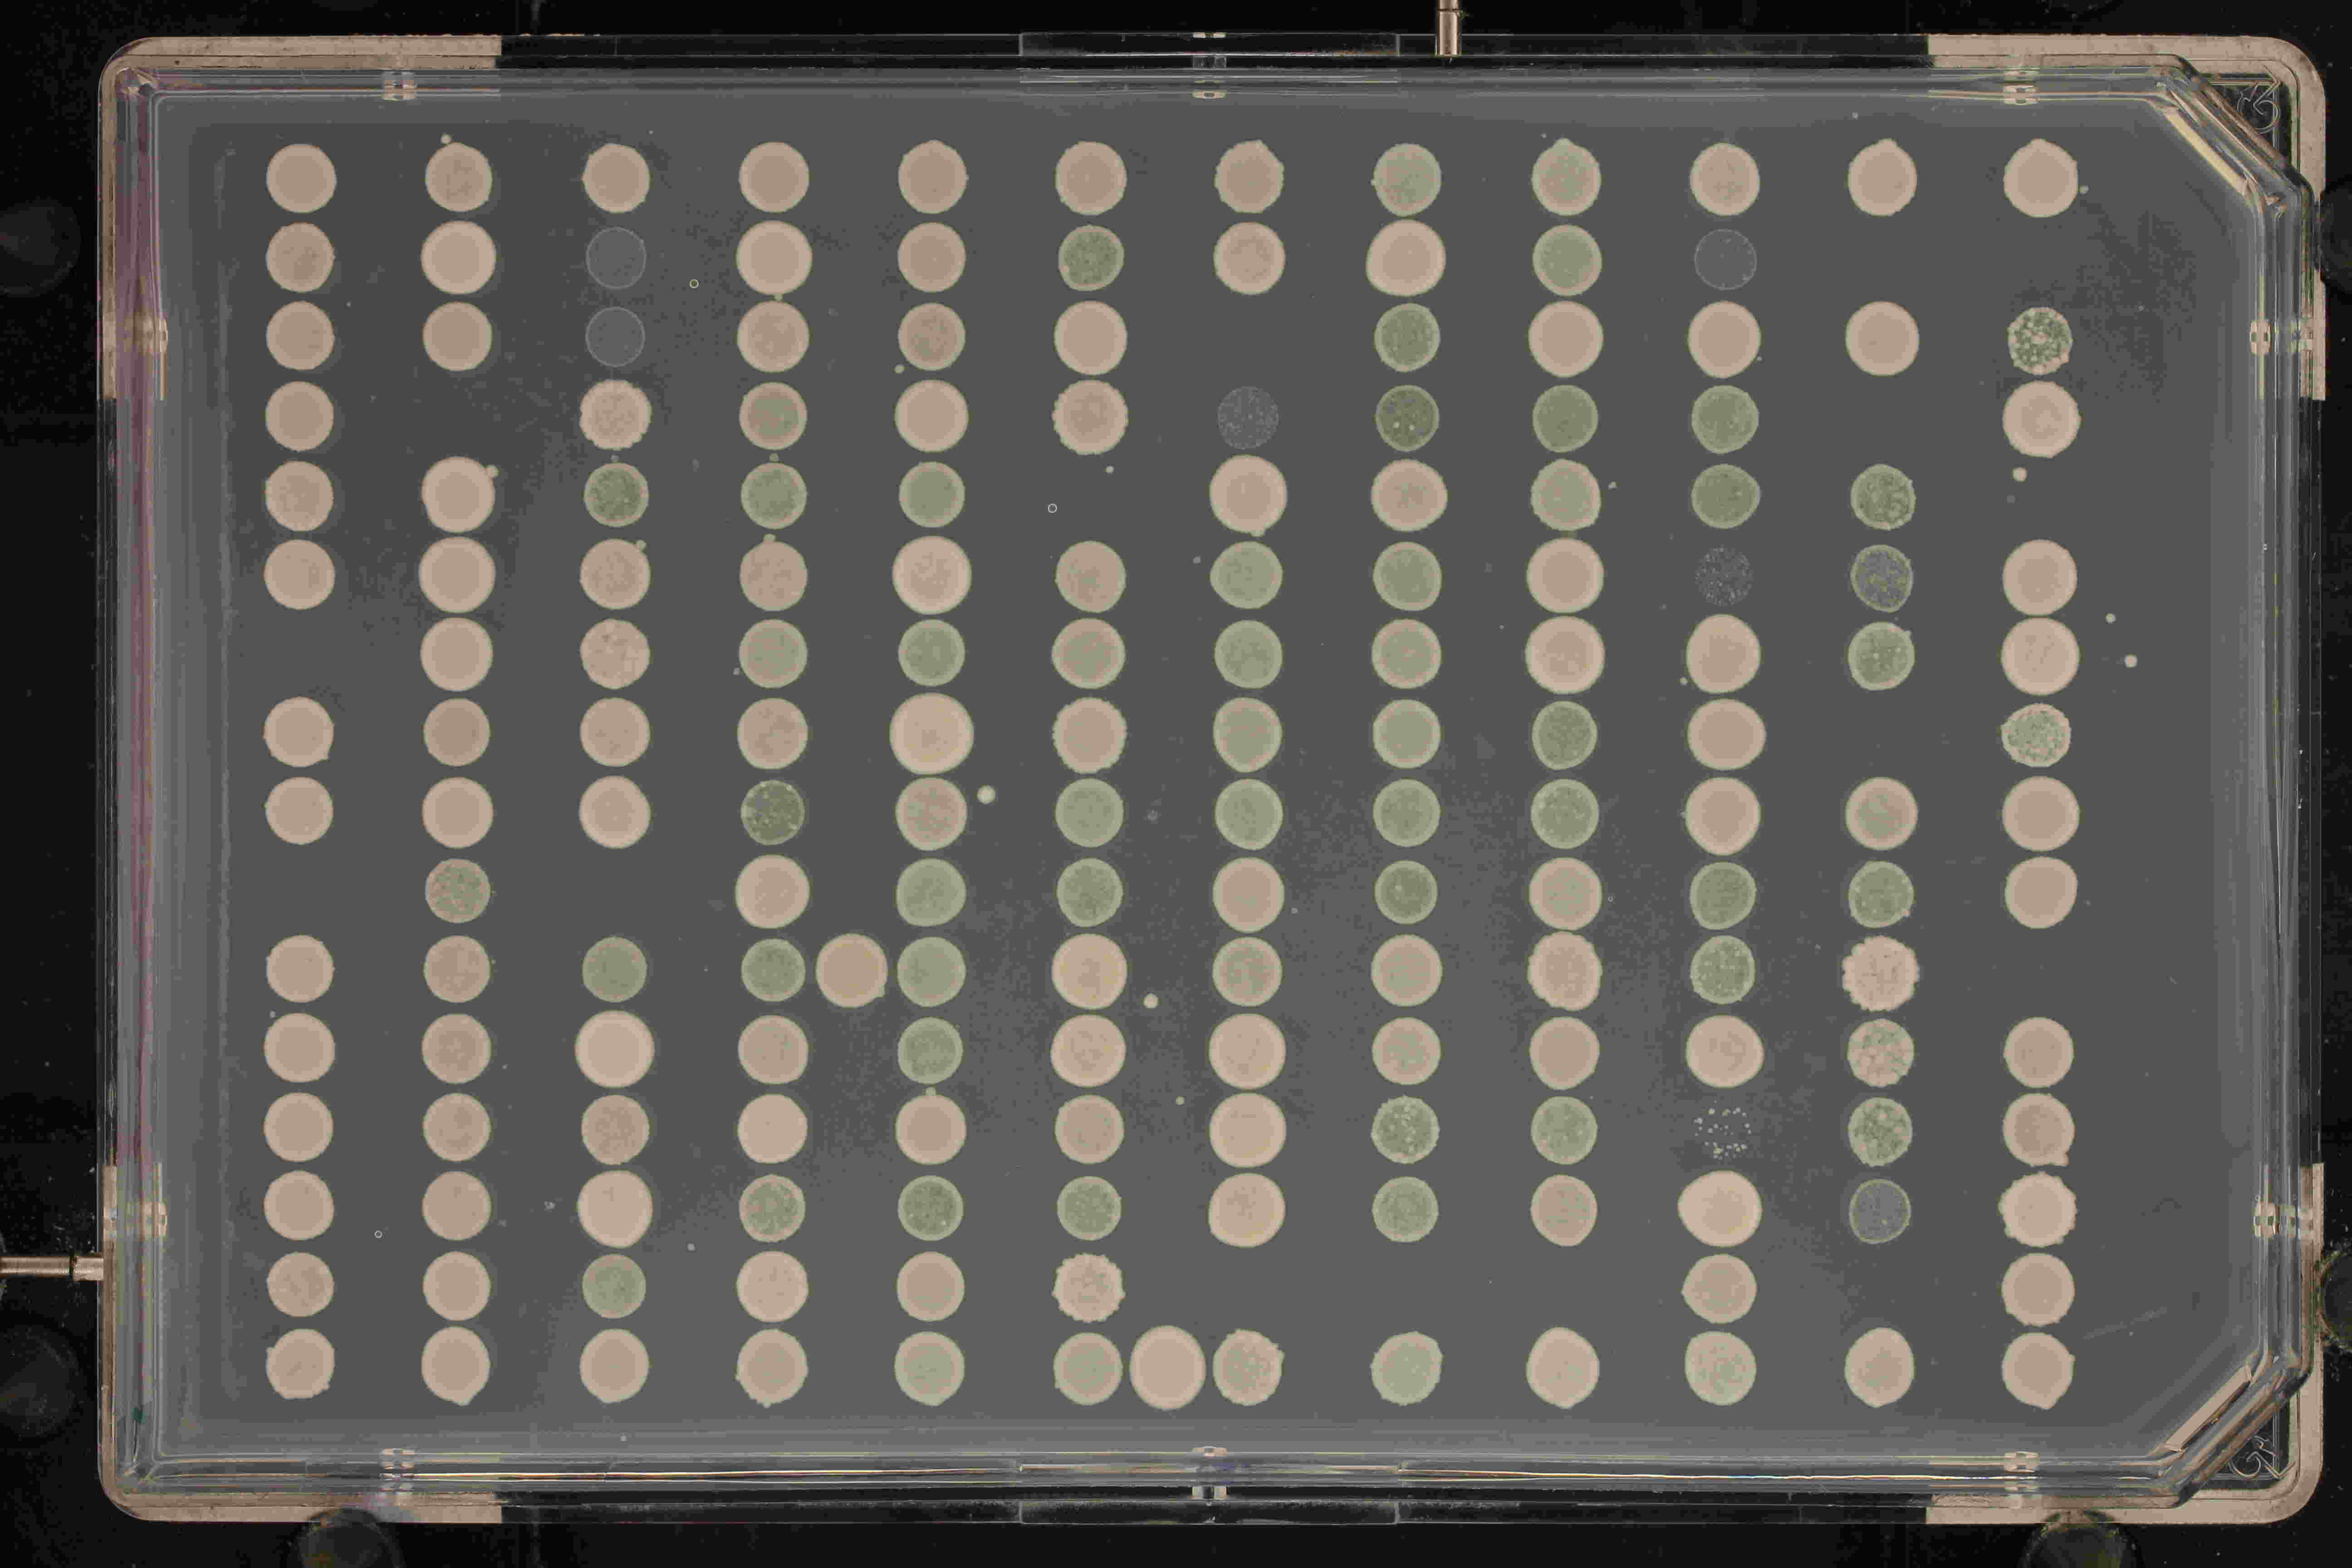
\includegraphics[width=\linewidth]{K000343_027_001_2015-02-21_19-38-08}
  \captionof{figure}{Schematics of diffusion across agar height.}
\end{Figure}

\subsection{Package and Distribute}
\label{sec:package-distribute}


%%% Local Variables:
%%% mode: latex
%%% TeX-master: "proposal"
%%% End:
